\justifying
\chapter{Results}
\label{chapter3}

<Results, evaluation (including user evaluation) {\em etc.} should be described in one or more chapters. See the `Results and Discussion' criterion in the mark scheme for the sorts of material that may be included here.>
\section{Performance}

% table for performance
\begin{table}[h]
    \centering
    \begin{tabular}{|c|c|c|}
        \hline
        \textbf{GPU} & \textbf{Texture Size} & \textbf{Time} \\
        \hline
        M1 & 256x256 & 4.97ms \\
        \hline
        M1 & 512x512 & 40.27ms \\
        \hline
        M1 & 1024x1024 & x-code didn't show performance \\
        \hline
    \end{tabular}
\end{table}

[FINISH THIS WHEN RESULTS RETRIEVED FROM UNIVERSITY]

\section{Comparison} 

\subsection{Spectrums}
The main diffrence comes to what kind of spectrum you use for FFT based oceans. The proposed "Phillips" spectrum \ref{fig:phillip_spectrum_comp} by \cite[J. Tessendorf]{tessendorf2001} has issues with energy transformation and following the wind direction. 
The proposed TMA spectrum \ref{fig:tma_spectrum_comp} handles energy transformation way more relistic and does not have any issues following the wind direction. This is mostly because that TMA is based on empirical data.
You can see clear diffrence between "Phillips" spectrum and TMA spectrum:

\begin{minipage}{0.48\textwidth}
    \centering
    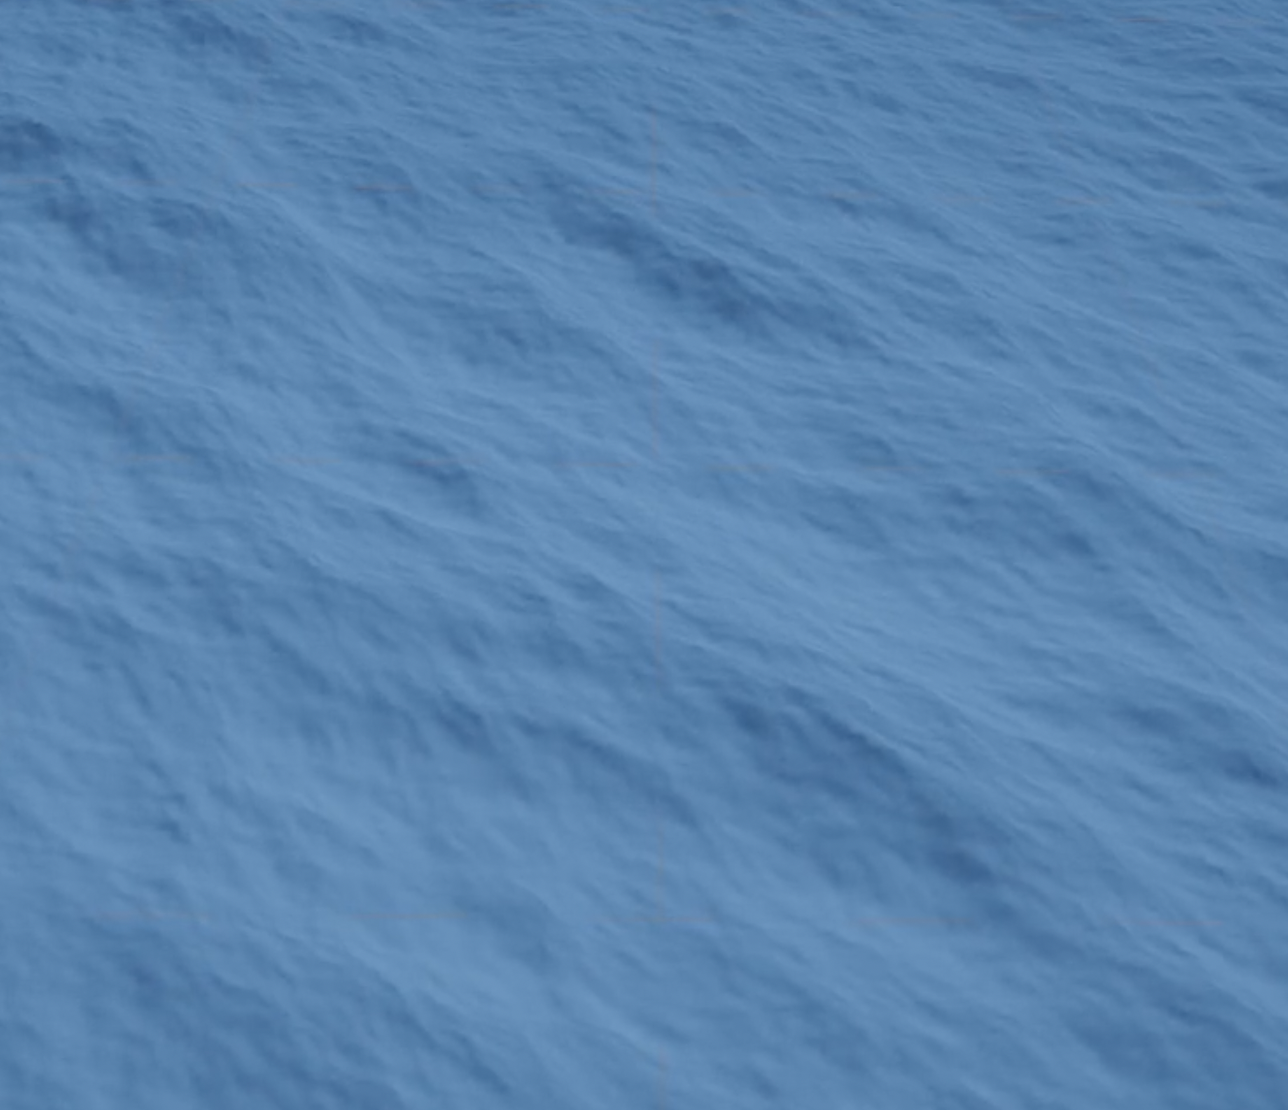
\includegraphics[width=0.8\textwidth]{"images/phillip_spectrum_comp.png"}
    \captionof{figure}{Height Map with $P_h$}
    \label{fig:phillip_spectrum_comp}
\end{minipage}
\hfill
\begin{minipage}{0.48\textwidth}
    \centering
    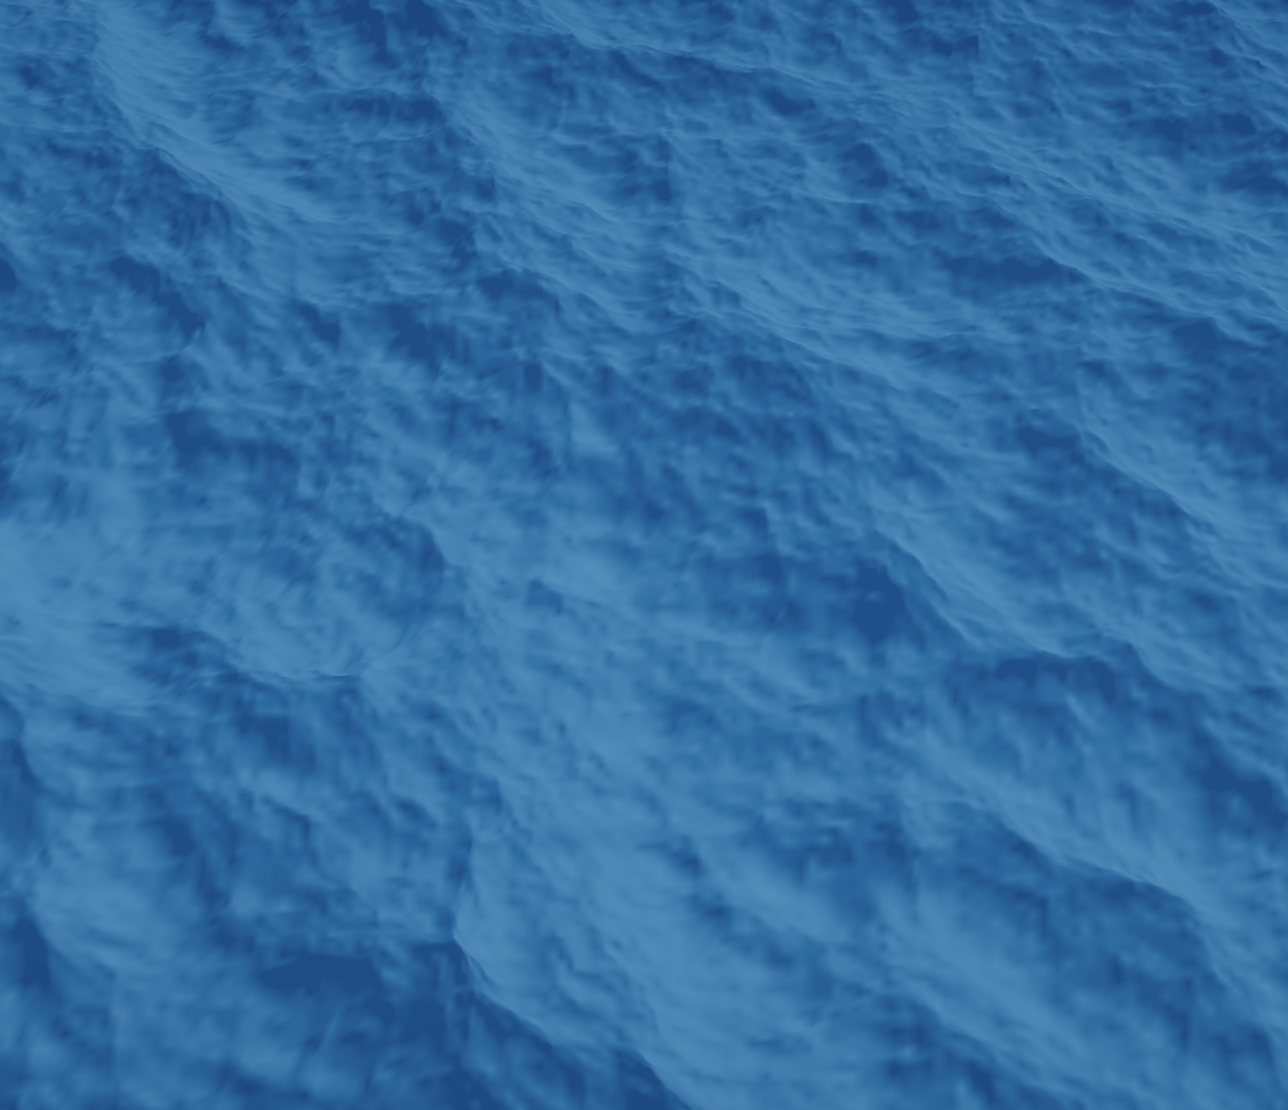
\includegraphics[width=0.8\textwidth]{"images/tma_spectrum_comp.png"}
    \captionof{figure}{Height Map using TMA Spectrum}
    \label{fig:tma_spectrum_comp}
\end{minipage}

\subsection{Real world oceans}
When it comes to calm ocean, the FFT based ocean with TMA spectrum performs extremelly well and holds the desired shape as shown in figures \ref{fig:real_calm_ocean} and \ref{fig:fake_calm_ocean}.
\begin{table}[h]
    \centering
    \begin{tabular}{|c|c|c|c|c|c|c|c|c|c|}
        \hline
        \textbf{Spectrum} & \textbf{Size} & $\mathbf{l_1}$ & $\mathbf{l_2}$ & $\mathbf{l_3}$ & $\mathbf{\lambda}$ & $\mathbf{U_{10}}$ & \textbf{Fetch} & \textbf{Depth} \\
        \hline
        256x256 & TMA & 256 & 100 & 10 & 0.9 & 0.02 m/s & 1000 km & 500 m \\
        \hline
    \end{tabular}
    \caption{Calm Ocean Parameters}
    \label{tab:calm_ocean}
\end{table}

\begin{minipage}{0.48\textwidth}
    \centering
    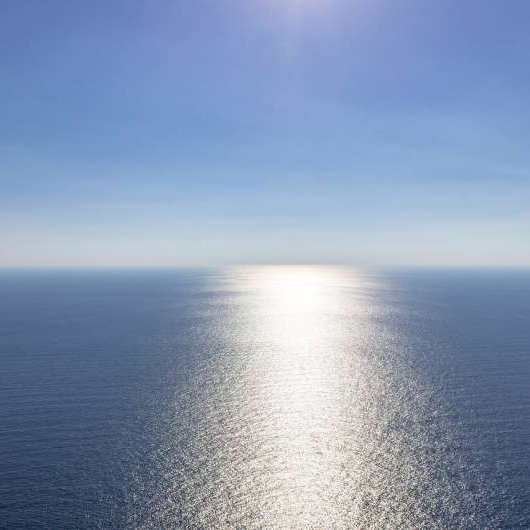
\includegraphics[width=0.8\textwidth]{"images/real_calm_ocean.jpg"}
    \captionsetup{justification=centering}
    \captionof{figure}{Calm Atlantic Ocean\\ Credits: CC0 Public Domain}
    \label{fig:real_calm_ocean}
\end{minipage}
\hfill
\begin{minipage}{0.48\textwidth}
    \centering
    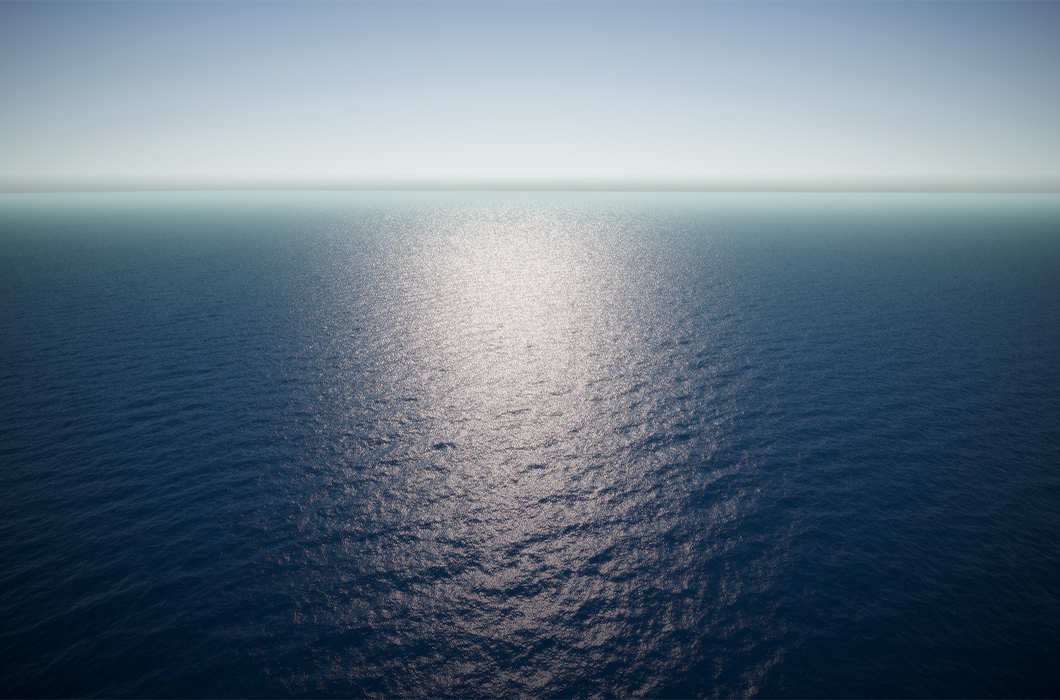
\includegraphics[width=0.8\textwidth]{"images/fake_calm_ocean.png"}
    \captionof{figure}{FFT Calm Ocean}
    \label{fig:fake_calm_ocean}
\end{minipage}

When it comes to stormy ocean where huge waves is expected the general shape of an ocean is still relistic
and can hadle the big waves without any trouble, and because of diffrent cascades the tilling is bearlly noticible as shown in the following figures \ref{fig:real_stormy_ocean} and \ref{fig:fake_stormy_ocean}.
\begin{table}[h]
    \centering
    \begin{tabular}{|c|c|c|c|c|c|c|c|c|c|}
        \hline
        \textbf{Spectrum} & \textbf{Size} & $\mathbf{l_1}$ & $\mathbf{l_2}$ & $\mathbf{l_3}$ & $\mathbf{\lambda}$ & $\mathbf{U_{10}}$ & \textbf{Fetch} & \textbf{Depth} \\
        \hline
        256x256 & TMA & 700 & 256 & 70 & 0.9 & 21 m/s & 1000 km & 500 m \\
        \hline
    \end{tabular}
    \caption{Stormy Ocean Parameters}
    \label{tab:stormy_ocean}
\end{table}
where each $l$ is the wave length scale of each cascade.

\begin{minipage}{0.48\textwidth}
    \centering
    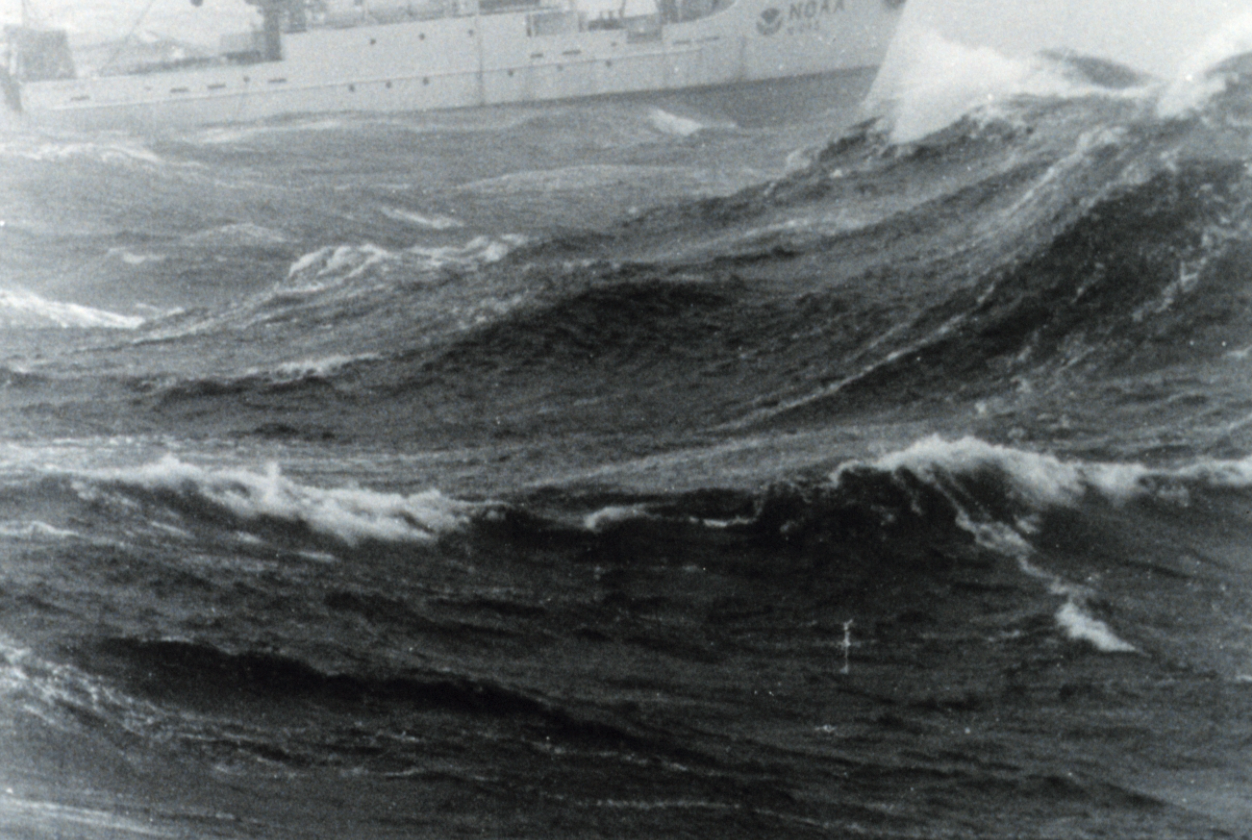
\includegraphics[width=0.8\textwidth]{"images/real_stormy_ocean.png"}
    \captionsetup{justification=centering}
    \captionof{figure}{Calm Atlantic Ocean\\ Credits: CC0 Public Domain}
    \label{fig:real_stormy_ocean}
\end{minipage}
\hfill
\begin{minipage}{0.48\textwidth}
    \centering
    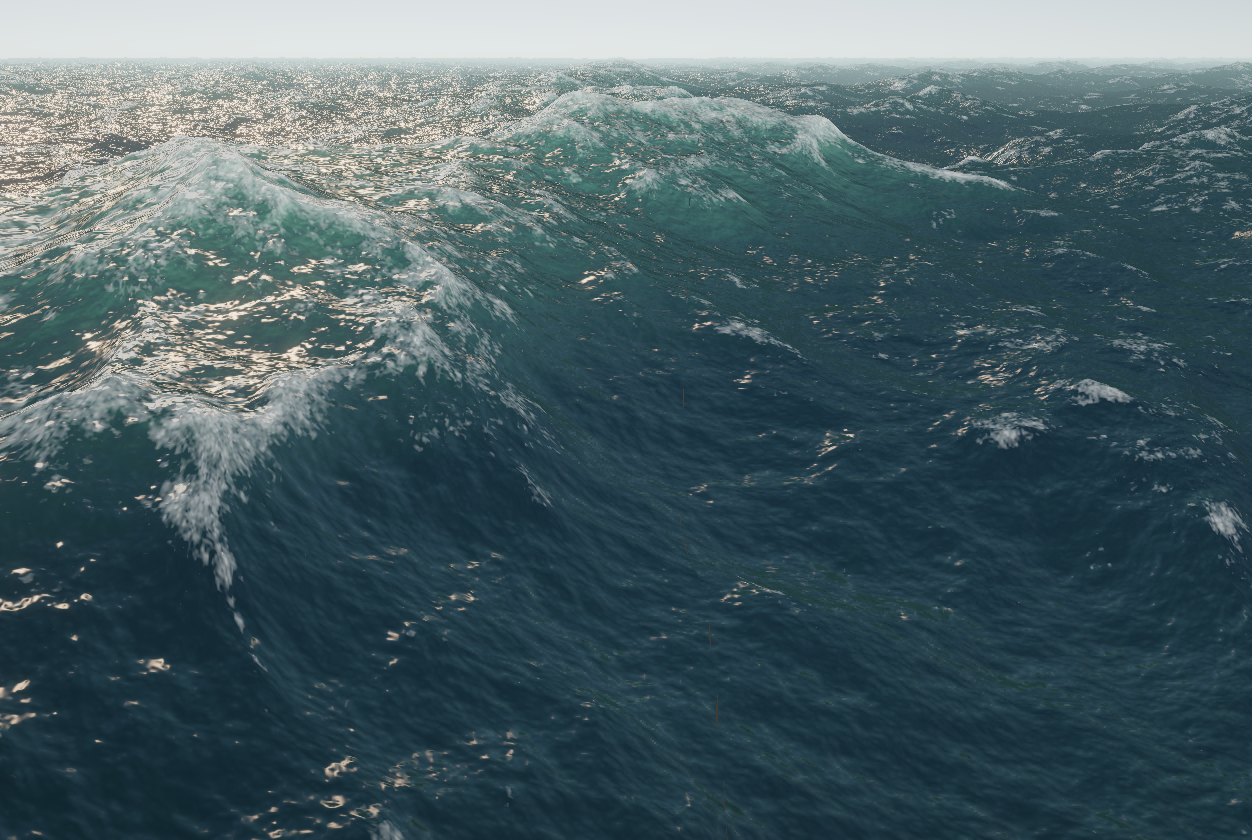
\includegraphics[width=0.8\textwidth]{"images/fake_stormy_ocean.png"}
    \captionof{figure}{Height Map using\\ TMA Spectrum}
    \label{fig:fake_stormy_ocean}
\end{minipage}

\section{Diffrent Outputs}

\section{Known Problems}